\documentclass[11pt]{article}

\usepackage{amsmath, amssymb, amsthm}
\usepackage{tikz}

\theoremstyle{plain}
\newtheorem{thm}{Theorem}[section]
\newtheorem*{thm*}{Theorem}
\newtheorem{prop}[thm]{Proposition}
\newtheorem{lem}[thm]{Lemma}
\newtheorem*{lem*}{Lemma}
\newtheorem{dfn}[thm]{Definition}
\newtheorem{cor}[thm]{Corollary}
\newtheorem{claim}[thm]{Claim}
\newtheorem{conj}[thm]{Conjecture}
\newtheorem{ques}[thm]{Question}
\newtheorem*{rem}{Remark}


\oddsidemargin  0pt
\evensidemargin 0pt
\marginparwidth 40pt
\marginparsep 10pt
\topmargin 0pt
\headsep 10pt
\textheight 8.2in
\textwidth 6.4in
\renewcommand{\baselinestretch}{1.1}

\newcommand{\codeg}{\text{codeg}}
\newcommand{\BBE}{\mathbb{E}}
\newcommand{\BFP}{\mathbf{P}}
\usepackage{amsmath}
\usepackage{amsthm}
\usepackage{amssymb}
\usepackage{mathtools}
\usepackage{hyperref}
\usepackage{url}





\usepackage{graphicx}
\usepackage{caption}
\usepackage{subcaption}

\def\eQb#1\eQe{\begin{eqnarray*}#1\end{eqnarray*}}
\def\eQnb#1\eQne{\begin{eqnarray}#1\end{eqnarray}}
\providecommand{\e}[1]{\ensuremath{\times 10^{#1}}}
\providecommand{\pb}[0]{\pagebreak}
\DeclarePairedDelimiter\ceil{\lceil}{\rceil}
\DeclarePairedDelimiter\floor{\lfloor}{\rfloor}

\newcommand{\E}{\mathrm{E}}
\newcommand{\Var}{\mathrm{Var}}
\newcommand{\Cov}{\mathrm{Cov}}

\def\Qb#1\Qe{\begin{question}#1\end{question}}
\def\Sb#1\Se{\begin{solution}#1\end{solution}}


\newtheoremstyle{quest}{\topsep}{\topsep}{}{}{\bfseries}{}{ }{\thmname{#1}\thmnote{ #3}.}
\theoremstyle{quest}
\newtheorem*{definition}{Definition}
\newtheorem*{theorem}{Theorem}
\newtheorem*{lemma}{Lemma}
\newtheorem*{question}{Question}
\newtheorem*{preposition}{Preposition}
\newtheorem*{exercise}{Exercise}
\newtheorem*{challengeproblem}{Challenge Problem}
\newtheorem*{solution}{Solution}
\newtheorem*{remark}{Remark}
\usepackage{verbatimbox}
\usepackage{listings}
\usepackage{mathrsfs}
\date{}
\title{\vspace{-0.7cm}
Limit Theorems II: Final}

\author{
Youngduck Choi 
\thanks{Department of Mathematics, Courant Institute of Mathematical Sciences, 
yc1104@nyu.edu; If you find an error and want to share with me, 
you can reach me via email.
}}

\begin{document}

\maketitle

\begin{abstract}
This work contains solutions for the final of the Limit Theorems II by Professor
McKean.
\end{abstract}


\begin{question}[1-1]
\hfill
\begin{figure}[h!]
  \centering
    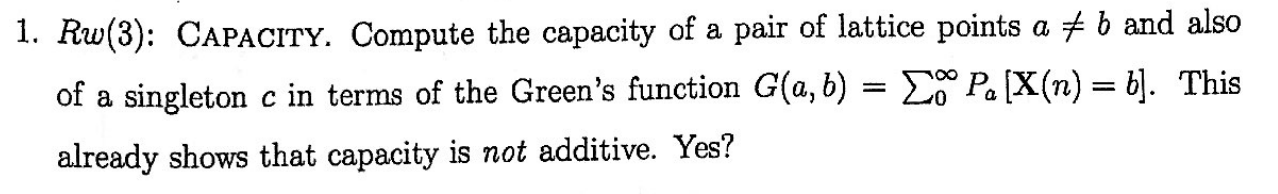
\includegraphics[width=0.7\textwidth]{limthm2-f-p1.png}
\end{figure}
\end{question}
\begin{solution} \hfill \\
Recall that for $K \subset \mathbb{Z}^3$ such that $|K| < \infty$, 
\eQnb
C(K) &=& \sum_{y \in \partial K} q(y) \>\>\> \text{with} \>\>\> q(y) = P_y(\{
X_n \not \in K \>\>\> \forall n > 0\}) \label{eq:1-1-1}
\eQne
Furthermore, for any $K \subset \mathbb{Z}^3$ such that $|K| < \infty$ and $x \in 
\mathbb{Z}^3$, we have Chung's formula from the textbook:
\eQnb
p(x) &=& \sum_{y \in \partial K} G(x,y) q(y) \label{eq:1-1-2}.
\eQne
where $p$ denotes the potential, which in particular equals $1$ on $K$.
Now, let $K = \{a,b\}$ such that $a \neq b$. Then, by~\eqref{eq:1-1-1},
\eQb
C(K) &=& q(a) + q(b)
\eQe
and by~\eqref{eq:1-1-2},
\eQnb
1 &=& p(a) = G(a,a)q(a) + G(a,b)q(b) \nonumber \\
1 &=& p(b) = G(b,a)q(a) + G(b,b)q(b) \label{eq:1-1-3} 
\eQne
By symmetry of RW(3), for any $x,y \in \mathbb{Z}^3$
\eQb
G(x,x) = G(0,0) \>\>\> \text{and} \>\>\> G(x,y) = G(y,x).
\eQe
Therefore, combined with~\eqref{eq:1-1-3},
\eQb
C(K) &=& q(a) + q(b) = \dfrac{2}{G(0,0) + G(a,b)}. 
\eQe
Similarly, let $K = \{a\}$ for some $a \in \mathbb{Z}^3$. Then, by~\eqref{eq:1-1-1},
\eQb
C(K) = q(a) 
\eQe
and by~\eqref{eq:1-1-2},
\eQb
1 = p(a) &=& G(a,a)q(a).
\eQe
Therefore,
\eQb
C(K) = \dfrac{1}{G(a,a)} = \dfrac{1}{G(0,0)}.
\eQe
Now, for any $x,y \in \mathbb{Z}^3$ such that $x\neq y$, define the canonical coordinate
path from $x \to y$ by first moving from $x$ to $(y_1, x_2, x_3)$, then to 
$(y_1, y_2, x_3)$, then to $(y_1, y_2, y_3) = y$. Notice that 
the number of timesteps required 
to move from $x$ to $y$ via the canonical path is $||x - y||_{1}$, which is finite. 
With this in mind, for any $x,y \in \mathbb{Z}^3$ such that $x \neq y$, 
\eQb
G(x,y) &=& \sum_{0}^{\infty} P_x(X_n = y) \geq P_x( X_n = y \text{ for some n} \geq 0)
\\
&\geq& P_x(\{ \text{the canonical coordinate path occurs} \}) 
= \dfrac{1}{6}^{||x-y||_1} > 0. 
\eQe
Then, for any $a,b \in \mathbb{Z}^3$, such that $ a \neq b$,
\eQb
C(a) + C(b) = \dfrac{2}{G(0,0)} &\neq& \dfrac{2}{G(0,0) + G(a,b)} = C(\{a,b\}), 
\eQe
which shows that $C$ is not additive. \hfill $\qed$


\end{solution}

\newpage

\begin{question}[1-2]
\hfill
\begin{figure}[h!]
  \centering
    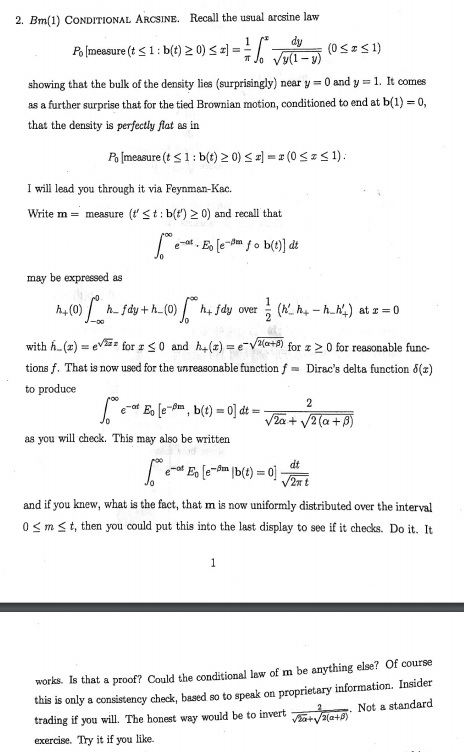
\includegraphics[width=0.7\textwidth]{limthm2-f-p2.png}
\end{figure}
\end{question}
\begin{solution} \hfill \\
Setting $f = \delta(x)$ as suggested, 
\eQb
\int_{0}^{\infty} e^{-\alpha t} E_0( e^{\beta \bold{m} 
(t)}, b(t) = 0) dt 
&=& \int_{0}^{\infty} e^{-\alpha t}  E_0(e^{-\beta \bold{m}} f \circ b(t)) dt ] \\ 
&=& \dfrac{h_+(0) \int_{-\infty}^{0} h_- f dy + h_- (0) \int_{0}^{\infty} h_+ f dy}{
\frac{1}{2} (h_{-}' h_+ - h_- h_{+}')|_{x = 0}} \\
&=& \dfrac{h_{+}(0) h_{-}(0) + h_-(0) h_+(0)}{\frac{1}{2} (\sqrt{2\alpha} + 
\sqrt{2(\alpha + \beta)})} = \dfrac{2}{\sqrt{2\alpha} + \sqrt{2(\alpha + \beta)}}. \\ 
\eQe
Now, assuming that $\bold{m}$ is uniform, we verify
\eQnb
\int_{0}^{\infty} e^{-\alpha t} E_0(e^{-\beta \bold{m}(t)} | b(t) = 0) \dfrac{dt}{
\sqrt{2\pi t}} &=& 
\int_{0}^{\infty} e^{-\alpha t} E_0( e^{\beta \bold{m} 
(t)}, b(t) = 0) dt \label{eq:1-2-1}  
\eQne
Observe that
\eQnb
\lim_{\epsilon \downarrow 0} \dfrac{1}{x} (e^{-(\alpha + \beta)x^2} - e^{-\alpha x^2} ))
|_{\epsilon}^{\infty} 
&=& \lim_{\epsilon \downarrow 0} \dfrac{1}{\epsilon} (e^{-(\alpha + \beta) \epsilon^2}
+ e^{-\alpha \epsilon^2}) = \lim_{\epsilon \downarrow 0} \beta \epsilon +  
O(\epsilon^3) = 0 \label{eq:1-2-2}
\eQne
where the second last equality holds via Taylor expansion. With the above limit in
mind we now compute  with $\bold{m} ~ \text{uniform}[0,t]$,
\eQnb
\int_{0}^{\infty} e^{-\alpha t} E_0(e^{-\beta \bold{m}(t)} | b(t) = 0) \dfrac{dt}{
\sqrt{2\pi t}}  
&=& \int_{0}^{\infty} e^{-\alpha t} \dfrac{1}{t\sqrt{2\pi t}}
\int_{0}^{t} e^{-\beta x} dx dt \nonumber \\
&=& \int_{0}^{\infty} e^{-\alpha t} \dfrac{1}{t\sqrt{2\pi t}}( \dfrac{1}{\beta}
- \dfrac{1}{\beta} e^{-\beta t}) dt \nonumber \\
&=& \dfrac{2}{\beta \sqrt{2\pi}} \int_{0}^{\infty} \dfrac{1}{x^2} e^{-\alpha x^2} 
- \dfrac{1}{x^2} e^{-(\alpha + \beta) x^2} dx \label{eq:1-2-3}\\
&=& \dfrac{2}{\beta\sqrt{2\pi}} (\lim_{\epsilon \downarrow 0} (
\dfrac{1}{x} (e^{-(\alpha + \beta)x^2} - e^{-\alpha x^2})|_{\epsilon}^{\infty}
\nonumber \\ 
&+& \sqrt{(\alpha + \beta)\pi} - \sqrt{\alpha \pi}) \label{eq:1-2-4} \\
&=& \dfrac{2}{\beta \sqrt{2 \pi}} (\sqrt{(\alpha + \beta)\pi} - \sqrt{\alpha \pi}) 
\label{eq:1-2-5}\\
&=&
\dfrac{(\sqrt{2(\alpha + \beta)} - \sqrt{2\alpha}}{\beta} = \dfrac{2}{\sqrt{2(\alpha
+ \beta)} + \sqrt{2\alpha}}, \nonumber  
\eQne
where~\eqref{eq:1-2-3} holds by a change of variables $t = x^2$,~\eqref{eq:1-2-4}
follows from integration by parts, and~\eqref{eq:1-2-5} holds by~\eqref{eq:1-2-2}.
This verifies~\eqref{eq:1-2-1}. This of course is not a complete proof as noted.
We have not yet proved that the uniform measure on $[0,t]$ is the ONLY measure
with such property. 
 \hfill $\qed$

\end{solution}

\newpage

\begin{question}[1-3]
\hfill
\begin{figure}[h!]
  \centering
    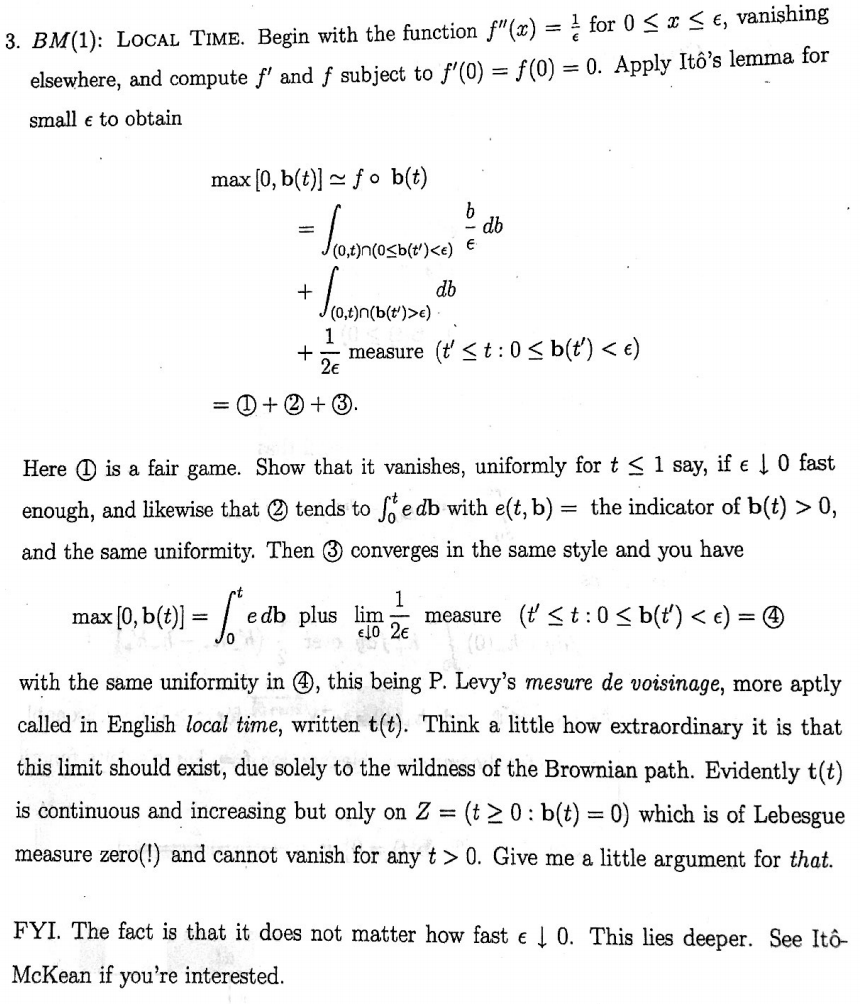
\includegraphics[width=0.7\textwidth]{limthm2-f-p3.png}
\end{figure}
\end{question}
\begin{solution} \hfill \\
Recall the Ito's formula for single martingales: If $f$ has enough regularity,
and for all $0 \leq t$,
\eQb
E\int_{0}^{t} [f'(M(s))]^2 dA(s) < \infty \>\>\> &\text{and}& \>\>\> E\int_{0}^{t} 
|f''(M(s))|dA(s) < \infty
\eQe
then, for all $0 \leq t$,
\eQnb
f(M(t)) - f(M(0)) &=& \int_{0}^{t} f'(M(s)) dM(s) + \dfrac{1}{2} \int_{0}^{t} 
f'(M(s)) dA(s) \label{eq:1-3-1}
\eQne
where $A(t)$ is the unique increasing, continuous process, corresponding to $M(t)$.
Of course, for the problem at hand, we have $M(t) = B(t)$ and $A(t) = t$, so $db(s)$ and
$ds$ will be used to denote the integrators. 
Now, to compute local time, we cannot naively apply this formula, as $\max(0,\cdot)$ is 
not $C^2(\mathbb{R})$. Hence, we approximate with the suggested strategy. 
Let $f_{\epsilon}$ be defined as given for each $\epsilon > 0$. Then, 
for any $0 \leq t$, and $\epsilon > 0$,
\eQnb
f_{\epsilon} \circ b(t) &=& f_{\epsilon} \circ b(t) - f_{\epsilon} \circ b(0) 
= \int_{0}^{t} f_{\epsilon}^{'}(B(s)) db(s) + \dfrac{1}{2} \int_{0}^{t}  
f_{\epsilon}^{''} (B(s)) ds \label{eq:1-3-2} \\ 
&=& \int_{\{s \in [0,t] : 0 \leq b(s) < \epsilon\}} \dfrac{b(s) }{\epsilon} db(s)
+ \int_{\{s \in [0,t] : b(s) > \epsilon\}} 1 db(s)
+ \dfrac{1}{2} \int_{ \{s \in [0,t] : 0 \leq b(s) < \epsilon\} } \dfrac{1}{\epsilon} 
ds  \label{eq:1-3-3} \\
&=& 
\int_{\{s \in [0,t] : 0 \leq b(s) < \epsilon\}} \dfrac{b(s) }{\epsilon} db(s)
+ \int_{\{s \in [0,t] : b(s) > \epsilon\}} 1 db(s) \nonumber 
+ \dfrac{1}{2\epsilon} \lambda_1( \{ s \in [0,t] : 0 \leq b(s) < \epsilon \}) \nonumber
\\ 
&=:& (I) + (II) + (III) \nonumber 
\eQne 
where~\eqref{eq:1-3-2} follows from~\eqref{eq:1-3-1},~\eqref{eq:1-3-3} follows
from definition of $f_{\epsilon}$ for each $\epsilon > 0$, and $\lambda_1$ denotes
1-dimensional Lebesgue measure as hinted. With the given fact that $(I)$ is a 
martingale, we claim that, for any $0 \leq t \leq 1$ uniformly, 
\eQnb
\int_{\{s \in [0,t] : 0 \leq b(s) < \epsilon\}} \dfrac{b(s)}{\epsilon} db(s) \>\>\> 
\text{converges to} \>\> 0 \label{eq:1-3-4}
\eQne
and
\eQnb
\int_{\{s \in [0,t] :  b(s) > \epsilon \}} 1 db(s) \>\>\> 
\text{converges to} \int_{0}^{t} e(s)  db(s)
\label{eq:1-3-5} 
\eQne
as $\epsilon \downarrow 0$ $\mathbb{P}$ almost surely. 
To show~\eqref{eq:1-3-4}, there exists a constant $C$, each $0 \leq t \leq 1$, for some
universal constant $C$, independent of $t$,
\eQnb
E\left[ \int_{0}^{t} \dfrac{b(s)}{\epsilon} 1_{\{0 \leq b(s) < \epsilon\}} - 0 db(s) 
\right]^2 
&=& E \int_{0}^{t} \left[ 
\dfrac{b(s)}{\epsilon} 1_{\{0 \leq b(s) < \epsilon\}} \right]^2 ds \label{eq:1-3-6} \\
&\leq& E \int_{0}^{t} 1_{\{ 0 \leq b(s) < \epsilon\}} ds \nonumber \\
&=& \int_{0}^{t} P(0 \leq b(s) < \epsilon) ds \nonumber \\
&=& \int_{0}^{t} P(0 \leq b(1) < \dfrac{\epsilon}{\sqrt{s}}) ds \label{eq:1-3-7} \\
&\leq& \int_{0}^{t} P(|b(1)| < \dfrac{\epsilon}{\sqrt{s}}) ds \leq C\sqrt{t} \epsilon
\label{eq:1-3-8},
\eQne
where~\eqref{eq:1-3-6} holds by the Ito $L^2$ isometry,~\eqref{eq:1-3-7} follows by 
the scaling of BW(1), and~\eqref{eq:1-3-8} follows from the fact that  
\eQb
\dfrac{P(|b(1)| \leq x)}{x} \>\>\> \text{is uniformly bounded } \>\>\> \text{for all} 
\>\>\> x > 0. 
\eQe
Hence, if $\epsilon = O(n^{-2})$, then, by Doob's inequality,
\eQb
(I) \to 0 \>\>\> \text{uniformly for } \>\>\> 0 \leq t \leq 1 \>\>\> P \>\>\> 
\text{almost surely}
\eQe
showing~\eqref{eq:1-3-4}. Now, denote the speed chosen above as $\gamma(n)$, which
is required to be $\lim_{n \to \infty} \gamma(n) = 0$ and 
$O(n^{-2})$. Now, by the Ito $L^2$ Isometry, for each $n$ and $0 \leq t \leq 1$, 
\eQnb
E\left[ \int_0^{t} (-1_{\{ b(s) > \gamma(n) \}} + 1_{\{b(s) > 0\}}) db(s) \right]^2
&=& E\left[ \int_0^t (-1_{\{b(s) > \gamma(n) \}} + 1_{\{b(s) > 0 \}})^2 ds \right] 
\nonumber \\
&=& E\left[ \int_{0}^{t} 1_{\{ \gamma(n) >  b(s) > 0  \}} ds \right] \label{eq:
1-3-5}.  
\eQne
Now, as $\gamma(n) \to 0$, for almost surely $w \in \Omega$, and
$n$ large enough
\eQb
1_{\{\gamma(n) > b(s)(w) > 0 \}} &=& 0 
\eQe
and hence
\eQnb
\int_{0}^{t} 1_{\{\gamma(n)> b(s)(w) > 0\}} ds &=& 0 \label{eq:1-3-6}
\eQne
Since, for each $n$,
\eQb
\int_{0}^{t} 1_{\{\gamma(n)> b(s) > 0\}} ds &\leq& 1_{ \{ [0,t] \times \{ \gamma(n)
> b(s) > 0 \}\}} \in L^1(\Omega\times[0,\infty))  
\eQe
by DCT on the product space, we see that the right hand side of~\eqref{eq:1-3-5}
converges to $0$, and
\eQb
\int_0^t 1_{\{ b(s) > \gamma(n)\}} db(s) \to 
\int_0^t 1_{\{ b(s) > 0\}} db(s) \>\>\> \text{in} \>\>\> L^2. 
\eQe
Hence, we can choose a subsequence of $\gamma(n)$, denote it as $\rho(n)$, such that
\eQb
\int_0^t 1_{\{ b(s) > \rho(n)\}} db(s) \to 
\int_0^t 1_{\{ b(s) > 0\}} db(s) \>\>\> \text{in} \>\>\> \text{almost surely}.  
\eQe
We see that uniformity of convergence persists by monotonicity ~\eqref{eq:1-3-6} with
$t$. Hence, we see that~\eqref{eq:1-3-4} and~\eqref{eq:1-3-5} holds by choosing
the speed $\rho(n)$ uniformly in $t \leq 1$. Now, for almost surely $w \in \Omega$,
and $m < n$,  
\eQnb
\left| \dfrac{1}{2
\rho(n)} 
\lambda_1( \{s \in [0,t] : 0 \leq b(s)(w) < \rho(n)\}) -
  \dfrac{1}{2
\rho(m)} 
\lambda_1( \{s \in [0,t] : 0 \leq b(s)(w) < \rho(m)\}) \right| \label{eq:1-3-7} 
\eQne 
is bounded above by
\eQb
\dfrac{1}{2\rho{(m)}}  
\lambda_1(\{s \in [0,t] : \rho(n)< b(s)(w) < \rho(m)\})  
\eQe
which in turn is bounded above by
\eQb
\dfrac{1}{2\rho(m)} \dfrac{2}{\pi} (\rho(m) - \rho(n)) = 
\dfrac{\rho(m) - \rho(n)}{\pi \rho(m)}  
\eQe
By choosing a subsequence of $\rho(n)$ of speed $O(2^{-n})$, $\psi(n)$, we see that
for almost surely $w \in \Omega$ and $m < n$,~\eqref{eq:1-3-7} is bounded above by 
\eQb
\dfrac{\psi(m) - \psi(n)}{\pi \psi(m)}  = O(2^{-m})
\eQe
and hence, for almost surely $w \in \Omega$,
\eQb
\dfrac{1}{2\psi(n)}\lambda_1(\{ s \in [0,t] : 0 \leq b(s)(w) < \psi(n) \} \>\>\>
\text{is cauchy, thus convergent}.
\eQe
Hence, we have established that with the sequence $\psi(n)$, the claimed convergence
of (I), (II), and (III) all hold. We are told that the convergence will hold for any 
speed, i.e. independent of the choice of the countable sequence converging to $0$,
but we will forgo the work for now.
From uniformity of convergence and continuity of Lebesgue measure, we see that
$\textbf{t}(t)$ is continuous, and clearly increasing as (II) and (III) are
increasing in t almost surely. In other words, for almost surely $w \in \Omega$, and
for all $t \geq s \geq 0$,
\eQb
\bold{t}(s)(w) \leq \bold{t}(t)(w). 
\eQe
To see that $\bold{t}$ only increases on $\{t : b(t) = 0\}$, consider
$|b(t)|$ as a semi-martingale with $t$ being its variance brocess. Then, applying
Ito's formula with $x^2$, 
\eQb
\int_{0}^{t} |B(s)| d\bold{t} &=& 0,
\eQe
which shows that $\bold{t}$ only increases at $\{t : b(t) = 0\}$. \hfill $\qed$

 
\end{solution}

\newpage

\begin{question}[1-4]
\hfill
\begin{figure}[h!]
  \centering
    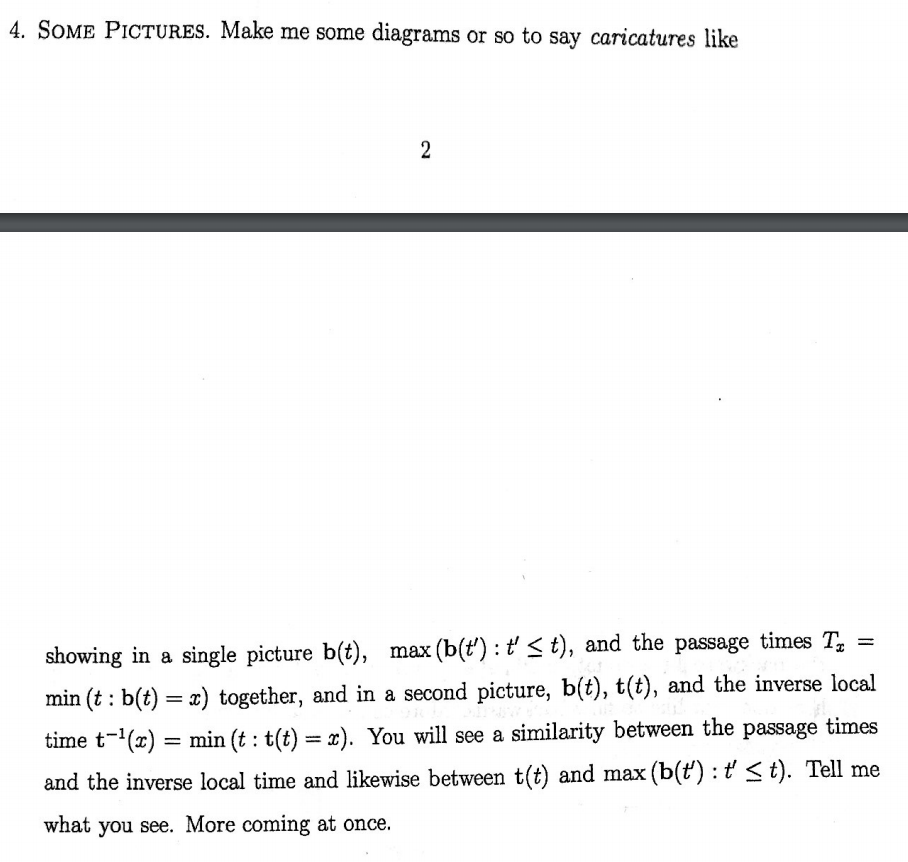
\includegraphics[width=0.7\textwidth]{limthm2-f-p4.png}
\end{figure}
\end{question}
\begin{solution} \hfill \\
Figures attached on the next page.

\end{solution}

\newpage

\begin{question}[1-5]
\hfill
\begin{figure}[h!]
  \centering
    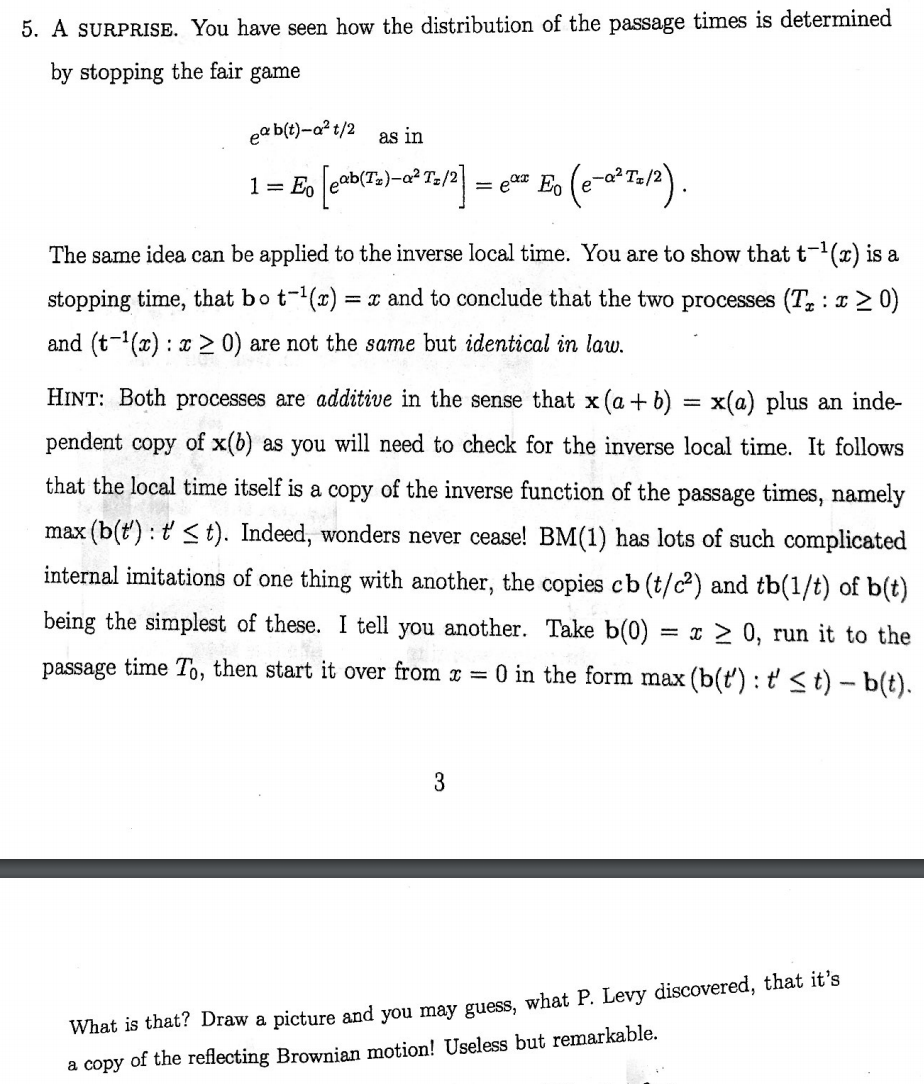
\includegraphics[width=0.7\textwidth]{limthm2-f-p5.png}
\end{figure}
\end{question}
\begin{solution} \hfill \\
Fix $x \in \mathbb{R}$. For any $t \geq 0$, 
\eQnb
\{w \in \Omega : 
\bold{t}^{-1}(x)(w) \leq t\} &=& 
\{ w \in \Omega: \bold{t}(\bold{t}^{-1}(x))(w) \leq
 \bold{t}(t)(w) \} \\
&=& 
 \{ w \in \Omega: x \leq
 \bold{t}(t)(w) \} \in \mathscr{F}_t \label{eq:1-5-1} 
\eQne
where~\eqref{eq:1-5-1} holds as $\bold{t}(\cdot)(w)$ is increasing
for almost surely $w \in \Omega$, 
and~\eqref{eq:1-5-2} holds as $\bold{t}(t)$ is $\mathscr{F}_t$ measurable.
By Optional Stopping time theorem,
\eQb
e^{\alpha x} E_0(e^{-\alpha^2 \frac{T_x}{2}}) &=& 
E_0(e^{\alpha b({T_x}) - \frac{\alpha^2 {T_x}}{2}}) = 1 \\
&=& E_0(e^{\alpha b(\bold{t}^{-1}(x)) - \frac{\alpha^2 \bold{t}^{-1}(x)}{2}})  
= e^{\alpha x} E_0(e^{-\alpha^2 \frac{\bold{t}^{-1}}{2}})
\eQe
Since the moment generating functions of $T_x$ and $\bold{t}^{-1}$ are the same any
$\alpha > 0$,
\eQb
T_x &=^{D}& \bold{t}^{-1},
\eQe
as required. \hfill $\qed$
\end{solution}

\newpage

\begin{question}[1-6]
\hfill
\begin{figure}[h!]
  \centering
    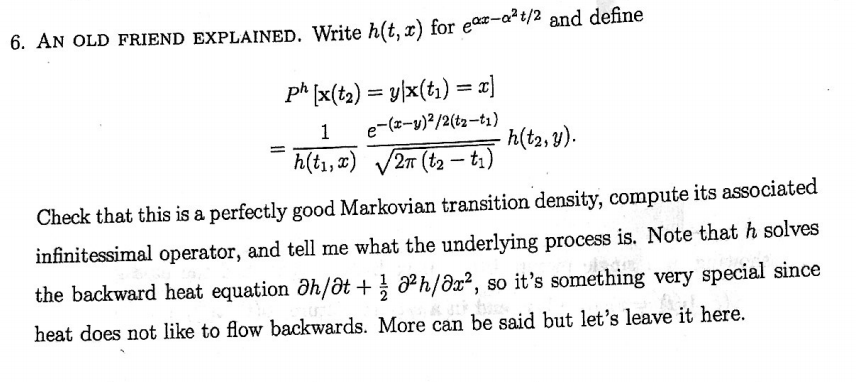
\includegraphics[width=0.7\textwidth]{limthm2-f-p6.png}
\end{figure}
\end{question}
\begin{solution} \hfill \\
We check that $P^h$ is a Markovian transition density by checking that it integrates
to 1 with respect to $y$. We compute, via completing the square,
\eQb
\int P^h(\bold{x}(t_2) = y | \bold{x}(t_1) = x) dy &=& \int
\dfrac{h(t_2,y)}{h(t_1,x)} 
\dfrac{e^{-(x-y)^2/2(t_2 - t_1)}}{\sqrt{2\pi(t_2 - t_1)}} dy \\
&=& \dfrac{1}{h(t_1,x)} \dfrac{1}{\sqrt{2\pi(t_2 -t_1)}} \int e^{-(y^2 - 2xy +x^2)/
2(t_2 - t_1) + \alpha y - \alpha^2 t_2/2} dy  \\
&=& \dfrac{1}{h(t_1,x)} e^{\alpha x - \frac{1}{2} \alpha^2 t_1} \int 
e^{\frac{-(y - (x + \alpha(t_2 - t_1))^2}{2(t_2 - t_1)}} dy  \\
&=& \dfrac{1}{h(t_1,x)} e^{\alpha x - \frac{1}{2} \alpha^2 t_1} = \dfrac{h(t_1,x)}{
h(t_1,x)} = 1.
\eQe
Now, we compute the associated infinitessimal operator.
Setting $s = t_2 - t_1$ and $t = t_1$, from the general theory, we 
know that the generator must be defined by
\eQnb
\mathscr{G} f(x) &=& \lim_{s \downarrow 0} \dfrac{\int f(y)P^h(
\bold{x}(t+s) = y | \bold{x}(t) = x) dy - f(x)}{s} \nonumber \\
&=& \dfrac{1}{h(t,x)} \lim_{s \downarrow 0} \dfrac{1}{s} 
\int f(y) \dfrac{e^{-\frac{(x-y)^2}{2s}}}{\sqrt{2\pi s}} h(t+s,y) dy - f(x)h(t,x) 
\nonumber \\
&=& \dfrac{1}{h(t,x)} \lim_{s \downarrow 0} \dfrac{1}{s} 
\int f(y) \dfrac{e^{-\frac{(x-y)^2}{2s}}}{\sqrt{2\pi s}} e^{\alpha y} e^{-\alpha^2 
\frac{(t+s)}{2}} dy - f(x)e^{\alpha x - \alpha^2 \frac{t}{2}} \label{eq:1-6-1} 
\eQne
whenever the limit is well-defined for $f \in C_0(\mathbb{R})$.
Recall that we saw from class that 
\eQb
u(s,x) &=& \int f(y) \dfrac{e^{\frac{-(x-y)^2}{\sqrt{2s}}}}{\sqrt{2\pi s}} e^{\alpha y}
dy  
\eQe
solves 
\eQb
u_t - \dfrac{1}{2}u_{xx} = 0 \>\>\> \text{and} \>\>\> u(0,x) = f(x) e^{\alpha x}.
\eQe
Therefore, we can continue~\eqref{eq:1-6-1} as
\eQb
&=& \dfrac{1}{h(t,x)} \lim_{s \downarrow 0} \dfrac{1}{s}
(u(s,x)e^{\frac{-\alpha^2 (t+s)}{2}} 
- u(0,x) e^{\frac{-\alpha^2 t}{2}} ) \\
&=& \dfrac{1}{h(t,x)} \lim_{s \downarrow 0} \dfrac{1}{s} 
((u(s,x) - u(0,x))e^{-\frac{\alpha^2(t+s)}{2}} + u(0,x)(e^{-\frac{\alpha^2(t+s)}{2}} 
- e^{-\frac{\alpha^2 t}{2}})) \\
&=& \dfrac{1}{h(t,x)} (\dfrac{1}{2} \partial_{xx} (f(x)h(t,x)) + f(x) \partial_t h(t,x))
\\   
\eQe
Hence, the generator of the process is 
\eQb
\mathscr{G} f = \dfrac{1}{h} ( \dfrac{1}{2} \partial_{xx} + \partial_t) (fh), 
\eQe
defined for each $f \in C(\mathbb{R})$ with 1-time partial and 2-space partials.
Furthermore, by noting that $h$ solves the backward heat equation, 
\eQb
\mathscr{G}f &=& \dfrac{1}{h} \partial_t h f + \dfrac{1}{2} \partial_x (f_x h 
+ h_X f) \\
&=& \dfrac{1}{h} \partial_{t} h f + \dfrac{1}{2h} (f_{xx} h + 2 f_x h_x + h_{xx} f) \\
&=& \dfrac{1}{2} f_{xx} + \dfrac{1}{h} h_x f_x, 
\eQe
and hence the underlying process $\bold{x}_t$ solves the stochastic differential 
equation
\eQb
d\bold{x}_t &=& \dfrac{\partial_xh(t,\bold{x}_t)}{h(t,\bold{x}_t)} dt + dB_t.
\eQe
\end{solution}
\end{document}
